\documentclass[11pt]{article}

% Impostazioni del documento
\usepackage[a4paper,top=2cm,bottom=2cm,left=1.5cm,right=1.5cm,marginparwidth=2.5cm]{geometry}
\usepackage{parskip} % Spazio tra i paragrafi
\usepackage{setspace} % Interlinea
\onehalfspacing% Interlinea 1.5

% Impostazioni del font
\usepackage{mathptmx} % Times New Roman
\usepackage[T1]{fontenc}

% Altri
\usepackage{multicol}
\usepackage{graphicx}
\usepackage{enumitem}
\usepackage{hyperref}
\hypersetup{
    colorlinks=true,    % Rendi i link colorati
    linkcolor=blue,     % Colore dei link interni (es. sezioni)
    citecolor=blue,     % Colore delle citazioni bibliografiche
    urlcolor=blue       % Colore degli URL
}

\usepackage[style=numeric, backend=biber]{biblatex}

\usepackage{listings}
\usepackage{graphicx}
\usepackage{xcolor}

\lstset{
  language=C++,
  backgroundcolor=\color{black!5}, % imposta il colore di sfondo
  basicstyle=\footnotesize, % imposta la dimensione del carattere di base
  breaklines=true, % consente la rottura automatica delle righe
  keywordstyle=\color{blue}, % imposta il colore delle parole chiave
  commentstyle=\color{green}, % imposta il colore dei commenti
  stringstyle=\color{red}, % imposta il colore delle stringhe
  numbers=left, % mostra i numeri di riga a sinistra
}


\addbibresource{Bib.bib} % Specifica il tuo file .bib

\begin{document}

\begin{titlepage}
    \centering
    
\includegraphics[width=0.5\textwidth]{aau.png}
    \vfill
    \begin{center}
        {\LARGE C++ for High-Performance Computing \par}
        \vspace{0.5cm}
        {\large Alessandro Castelli [12246581] \par}
        \vspace{0.5cm}
        {\large \today \par}
    \end{center}
    \vfill
\end{titlepage}

\begin{multicols*}{2}[\columnsep=1cm]
    
    \section{Introduction}
    In this paper, we will analyze and discuss three articles that delve into the usage of the \texttt{C++} programming language in the realm of high-performance computing.

    The selected articles provide diverse perspectives on the topic, and they are as follows:
    \begin{enumerate}
        \item \textit{C++ Reflection for High Performance Problem Solving Environments}~\cite{Article1}, available at: \href{https://citeseerx.ist.psu.edu/document?repid=rep1&type=pdf&doi=2058bb40e6b80504ba1084452fd9c126cd19f891}{https://citeseerx.ist.psu.edu}
        \item \textit{How Templates Enable High-Performance Scientific Computing in C++}~\cite{Article2}, available at: \href{https://ieeexplore.ieee.org/abstract/document/774843?casa_token=YqZfo7t12KoAAAAA:aUt-msPVNEAtzfVwO4h_-R_r7IPTFs7vHYHbAtsOdDE83PlNvB8gkNl5maWpHYBU5QkS3cUp0R8}{https://ieeexplore.ieee.org}
        \item \textit{Conduit: A C++ Library for Best-Effort High Performance Computing}~\cite{Article3}, available at: \href{https://dl.acm.org/doi/abs/10.1145/3449726.3463205}{https://dl.acm.org}
    \end{enumerate}

    Each of these documents addresses challenges in high-performance environments. Specifically, the first article introduces a reflection system for the C++ language, enabling dynamic manipulation of program objects and functions during runtime. The second article discusses the use of C++ in developing flexible and high-performance scientific code, leveraging the powerful capabilities of templates. The third article introduces \texttt{Conduit}, a C++ library that provides an interface for implementing software using "best-effort" inter-thread and inter-process communication. The concept of "best-effort" is a strategy that reduces hardware synchronization and reliability requirements, accepting nondeterminism in exchange for efficiency.

    In the following sections of the document, we will delve into the topics covered in each article, along with their methodologies, results, and critical considerations on the proposed implementations.

    \section{C++ Reflection for High-Performance Problem Solving Environments}
    The article discusses the importance of Problem Solving Environments (PSE), which are computing systems that provide the necessary resources to solve specific classes of problems. These PSEs should include advanced problem-solving methods, automatic or semi-automatic method selection, and the ability to incorporate new approaches. In scientific computing, PSEs must tackle CPU-intensive tasks, often developed as components in high-performance languages.
    
    The article argues that PSEs should allow for \textbf{dynamic task coupling}, either through a graphical user interface or a scripting environment. However, the lack of reflection\footnote{Reflection in programming languages refers to the ability of a program to examine and modify its structure and behavior during runtime. In practice, a reflective programming language allows the program to "look at itself" and make dynamic changes to its execution. This concept is mainly divided into type reflection, which concerns the dynamic analysis of data types, and data reflection, which deals with the dynamic manipulation of data during execution.} in modern HPC languages leads PSE developers to rely on languages like Java, causing inconveniences.
    \textbf{The article proposes the implementation of non-intrusive and standards-compliant reflection features (in a library) in C++}, demonstrating that this can be done efficiently. It compares the overhead of reflection with other methods and suggests that its implementation is the only way to incorporate reflection features in C++ in a standards-compliant and non-intrusive manner.
    
    The article discusses two types of code-level reflection: compile-time and runtime reflection. Compile-time reflection allows access to type information during compilation, facilitating generic programming, while runtime reflection provides the ability to dynamically access type information during program execution.
    
    While languages like Java, C\#, and Python support reflection as part of their standard specifications, C++ provides only limited functionality through runtime type information (RTTI). Visual C++ has extensions for reflection but with limited portability. For high-performance computing, Java and C\# are limited, Fortran dominates, but C++ is preferred for middleware.
    
    Runtime reflection requires the separate generation of metadata as actual C++ code since C++ compilers do not automatically generate the required metadata. The article proposes that C++ should support reflection in a standard and non-intrusive way, and demonstrates how this can be efficiently achieved.
        
    \paragraph{Example taken from the document:}
    Consider the following code block:
    \begin{lstlisting}
        classType = ClassType::getClass("Service1");
        obj = classType.createInstance();
        obj.invoke("method1");
    \end{lstlisting}
    
    The use of reflection allows dynamically incorporating existing modules into an application in a dynamic and flexible manner. For instance, considering a function like \texttt{init\_lib()}, it would typically require writing specific code, but with reflection, one can specify the function name in a configuration file, enabling dynamic invocation without the need to write new code or recompile. This approach extends to other functions of the module, allowing automatic glueing between modules through the use of an ontology or semantic description. Reflection thus becomes a powerful tool for developing reusable code, simplifying the process of integrating existing modules into a larger application. By making "Service1" and "method1" configurable parameters, this code could be used to invoke any method.
    
    The major advantages in this are:
    \begin{itemize}
        \item \textbf{Dynamic Configurability:} Using reflection, it's possible to dynamically specify which classes and methods should be used without modifying the source code. For example, in the provided code block, the class name ("Service1") and method name ("method1") can be specified in a configuration file rather than in the code.
        \item \textbf{Integration of External Modules:} Reflection simplifies the integration of external modules or libraries into an application without the need to adapt existing source code. This makes it easier to add, remove, or replace functionality without recompiling the main application.
        \item \textbf{Code Reusability:} Reflection can promote writing more generic and reusable code. In the case of functions like "init\_lib()", the ability to dynamically call functions based on their name simplifies the usage of modules without writing specific code for each function.
        \item \textbf{Ease of Update and Maintenance:} If reflection is used to dynamically manage application features, updating or modifying parts of the application can become simpler without impacting other parts of the code.
    \end{itemize}
    \paragraph{Reflection: Ideas on How It Can Be Applied}
    The document provides various ideas on how to apply reflection using different techniques. Below, you will find different contexts and use cases where reflection is implemented or leveraged to achieve specific advantages or functionalities.
    
    \begin{itemize}
        \item \textbf{Serialization:}
        The serialization process, which involves converting the state of an object into a sequence of bytes and subsequently deserializing it, is a common method for communication between loosely coupled applications. In the context of a PSE, this byte sequence can be used to transfer data from the output of one task to the input of another. By using reflection, the sender can dynamically serialize the state of an object and send it to the receiver, who can dynamically create objects based on their descriptions and populate them with corresponding state information.
        
        \item \textbf{Scripting Environment Interface:}
        In the context of reflection and interfacing with a scripting environment, the goal is to allow users of a scripting language, such as Python, to use functionalities implemented in high-performance languages like C, C++, or Fortran without the need to completely rewrite the code in a scripting language. High-performance libraries, written in languages like C, C++, or Fortran, are often used for intensive computational tasks or performance optimization. However, direct access to these libraries by users who prefer scripting languages like Python might be complex due to differences in memory management, syntax, and language structure. Reflection is used to create an interface between these libraries and the scripting environment. Instead of requiring scripting users to write complex wrappers or bindings to call functions from these libraries, reflection is employed to provide a more automatic and less burdensome mechanism.
    
        \item \textbf{Object Instantiation:}
        Reflection is employed to address the issue of polymorphic object instantiation, providing an alternative to the need for a specific factory method for each class. This approach makes the instantiation process more flexible and less intrusive. In the context of polymorphic instantiation, the common practice is to use the factory method pattern, which requires each candidate class to implement a dedicated method for creating a new object of the required type. This procedure can be cumbersome and intrusive, especially when working with new classes or existing classes that need adaptation. With the use of reflection, the constraints of the factory method pattern are not required. Instead, objects can be instantiated dynamically without the need to implement specific factory methods.
    \end{itemize}

    \paragraph{Objectives of the Reflection Library in C++}
    \begin{enumerate}
        \item \textbf{Runtime Access to Members:} Provide the ability to access class member functions and data members at runtime, enabling the invocation of member functions and reading/writing of data members.
    
        \item \textbf{Completeness:} The library should offer comprehensive information about classes and their members, allowing detailed access.
    
        \item \textbf{Standard Compliance:} Be compliant with the ISO C++ standard, ensuring the portability of the library without relying on non-standard features.
    
        \item \textbf{Efficiency:} Minimize the overhead of accessing classes and their members through reflection. The use of C++ templates to record most metadata at compile-time contributes to ensuring efficient resulting code.
    
        \item \textbf{Non-Intrusiveness:} Implement reflection without requiring modifications to existing code. Avoid adding special annotations to existing classes to ensure easy integration with existing code and reduce the risk of errors in metadata sections.
    \end{enumerate}

    \subsection{Implementation of the Reflection Library in C++}
    The library is structured with a core of basic classes and a set of generated classes to handle type-specific information. These type-specific metadata classes are created by parsing user-provided target classes and processing their syntax trees. This approach allows us to efficiently store and present reflection information without being intrusive and ensuring compliance with C++ language standards.
    
    \paragraph{Metaclasses}
    \texttt{ClassType} è la metaclasse utilizzata per rappresentare classi definite dall'utente. 
    Queste classi derivano da una classe più generica chiamata \texttt{Type} (Guarda figura \ref*{fig:ClassType}).
    
    \texttt{ClassType}, along with its supporting classes, provides the following features:
        \begin{itemize}
            \item Name and type
            \item List of data members and member functions
            \item Instantiation interface
            \item Inheritance information
        \end{itemize}
    After creating an instance of \texttt{ClassType}, the actual target object can be instantiated.
    The other derived types, \texttt{FundamentalType}, \texttt{ArrayType}, and \texttt{PointerType}, as their names suggest, are used to represent primitive types (e.g., integer, double), arrays, and pointers.

    \subsection{Member Classes}
    There are two types of member classes, namely, data members and member functions. These encapsulate the members of a class and provide means to access them indirectly, given their name at runtime. Instead of maintaining the offset to the encapsulated member, each member class keeps a pointer to its respective data member or member function. This ensures that this library is fully compliant with the C++ standard.
    \subsubsection*{Data Members}
    Each data member in a class is represented by a DataMember object. This object contains information such as name and type.
    The ref() method returns a reference to the represented object, allowing the program to manipulate it as if it had direct access to the data member.
    BoundDataMember is aware of the associated object, eliminating the need to pass a reference to classAObj. Bound data members are now completely independent of the underlying type, making them suitable for fully generic code.
    \subsubsection*{Member Functions}
    Member functions are represented by the \texttt{MemberFunction} classes, providing information such as name, return type, and additional interfaces.
    The arguments of member functions are handled as a vector of generic Type objects, allowing the representation of fundamental types, pointers, arrays, and user-defined classes.
    Invocation of member functions can occur in two ways: one requires sending arguments individually with a pointer to the corresponding instance, and the other accepts a vector of arguments.

    \subsection{Performance}
    After the implementation of the library, tests were conducted to evaluate its performance. A performance drop was expected, and the goal was to measure the time increase compared to direct calls. Each test involved the dynamic instantiation of an object and the invocation of a method on it, with five methods varying in the number of arguments (from 1 to 5). The methods were invoked as both direct and virtual calls, as well as using reflection. In the case of reflection usage, the object instance was created using reflective methods. The main focus was on detecting the overhead in reflection usage compared to direct calls, calculating this overhead as the additional time in percentage compared to direct calls.
    
    What can be observed from the tests is that the overhead for reflection in C++ increases with the number of arguments. This is mainly due to the dynamic construction of the argument list, which involves a few small memory allocations.
    
    \subsection{My Vision}
    The development of this library, in my opinion, presents several interesting insights. Below, I will list some points summarizing my vision with potential improvements.
    
    \begin{itemize}
        \item \textbf{Enrichment of Features:} The primary goal is to enrich the reflection library by introducing new features that enhance its power and extensibility. In this context, careful consideration is given to including support for handling custom attributes, implementing advanced class hierarchy navigation, and developing tools for advanced type manipulation.
        \item \textbf{Performance Optimization:} Special attention is devoted to performance optimization with the aim of further reducing the overhead introduced during the invocation of member functions and access to data members. Maintaining a constant focus on efficiency, we aim to ensure that the library can be used in high-performance contexts without compromising its efficiency.
        \item \textbf{Integration with External Technologies:} Actively explore opportunities for integration with widely adopted technologies and frameworks. The library could benefit from increased compatibility with popular serialization/deserialization systems or scripting environments, opening up new possibilities for usage in complex and heterogeneous scenarios.
        \item \textbf{Wide Compiler Support:} Commitment to ensuring that the library is compatible with a broad range of C++ compilers. The goal is to extend support beyond the currently considered compilers, ensuring the library is accessible to a broader audience of developers using various development environments.
        \item \textbf{Comprehensive and Accessible Documentation:} Investment in creating comprehensive, clear, and accessible documentation. The documentation will be enriched with practical examples, detailed use-case scenarios, and technical explanations. This effort aims to guide developers, both beginners and experts, in the effective use of the library, contributing to its adoption and success in the community.
        \item \textbf{Rigorous Testing and Validation:} Implementation of a comprehensive testing and validation system to ensure the library functions correctly in various situations and configurations. Through this rigorous approach, the goal is to maintain the stability and reliability of the library over time, providing developers with the necessary confidence in integrating and using the library.
    \end{itemize}

    \section{How templates enable high-performance scientific computing in C++}
    The C++ programming language provides a powerful template framework, allowing the development of flexible software without sacrificing performance. Templates enable the definition of parameterized classes and functions in terms of other types and constants. This feature is crucial for building abstract and high-performance scientific codes in C++. The Pooma framework is cited as an example, supporting high-performance scientific computing and providing advanced mathematical and physical abstractions.
    
    Pooma allows for a smooth transition between serial and parallel execution on different platforms, including supercomputing.
    
    \paragraph{How templates work in C++}
    Below, you will find a simple example of how templates can be useful.
    \begin{lstlisting}[language=C++, label=code1, caption={Max function without template}]
    if (a > b) return a;
    else return b;
    \end{lstlisting}
    If we needed to write a version for float, double, or any other arithmetic type, the code would be exactly the same. Instead of reproducing this code for every type, we can write a template function (Listing \ref{code2}) to generate a more general function.
    
    \begin{lstlisting}[language=C++, label=code2, caption={Max function with template}]
    template <class T>
    T max(T a, T b)
    {
    if (a > b) return a;
    else return b;
    }
    \end{lstlisting}
    
    The symbol T is a template parameter in C++, and the syntax "class T" can be misleading because T does not necessarily have to represent a C++ class. Template arguments can be explicitly specified, for example, with `max<int>(3, 2)`, where the compiler creates a concrete version of max by substituting int for T. However, it is more common to allow the compiler to deduce the type by observing the arguments, as in the case of `max(3.0, 2.0)`, where the compiler will generate a version of max with double substituted for T.
    This type deduction is not a simple textual substitution, as would occur with a macro preprocessor. T is expected to have the semantics of a type, allowing the declaration of objects of that type, as highlighted in the function arguments and return value of the max function. In summary, the use of templates in C++ allows for significant flexibility in creating generic functions and classes, with compiler type deduction contributing to the simplicity and clarity of the code.

    \subsection{Pooma}
    \paragraph{Array Concept}
    When used alone, an array refers to all values within its domain to which mathematical operations or elementary functions can be applied. An array in Pooma can have up to seven dimensions and can serve as containers for arbitrary types.
    The Array concept in Pooma supports more complex domains, and furthermore, the indexing of arrays in Pooma is polymorphic. That is, the indexing operation \texttt{X(i1, i2)} can perform the mapping from domain to range in various ways, depending on the specific type of the array being indexed.
    Let's delve into the Array concept model in Pooma, specifically the class template Array.
    The three most important design considerations are:\\
    • Arbitrary domain,\\
    • Arbitrary range, and\\
    • Polymorphic indexing.\\
    The class template Array in Pooma allows for the creation of different Array classes, each with a different number of dimensions (Dim), element type (T), and indexing mode (EngineTag). This flexibility enables the definition of arrays with arbitrary domains, arbitrary output ranges, and different indexing modes, contributing to a versatile and efficient overall design.
    
    \paragraph{Engine}
    The concept of "Engine" in Pooma is fundamental for polymorphic indexing in the management of multidimensional arrays. The "Array" class delegates the storage and retrieval of data to an "Engine" object, whose design is driven by specific requirements to be considered a model of the Engine concept.

    The "Array" class is parameterized by three templates: Dim (domain dimension), T (type of array elements), and EngineTag (indexing mode). This parameterization allows the creation of different Array classes with specific characteristics, promoting a flexible and efficient design.

    The concept of Engine is defined by the requirements imposed by the Array class on its engine. In particular, the engine must be a specialization of a general template "Engine" with parameters identical to those of the Array class. It must also publicly define a type called "Index\_t" and provide a version of the "()” operator that accepts indices of type "Index\_t".

    The indirection between Array and Engine allows Pooma to support polymorphic indexing. For example, if the engine works with a discrete domain, it defines "Index\_t" as an integral type; if it works with a continuous domain, it defines "Index\_t" as a floating-point type.

    The "Array" class uses the "()” operator to pass indices to its "Engine" object. This separation allows Array to be a faithful model of the Array concept, offering a wide variety of constructors, overloaded operators, and support for expressions. In contrast, Engine objects are a low-level interface to a user-defined data source, providing direct access to data managed by Array.

    Pooma's approach, based on the separation of interface and implementation, provides greater complexity and feature richness in the Array class compared to Engine objects, allowing easy extension and customization by users.


    \subsection{Compile-time versus runtime polymorphism}
        The comparison between compile-time and runtime polymorphism highlights crucial differences in terms of flexibility and efficiency in implementing the Engine concept in Pooma. The article emphasizes compile-time polymorphism, emphasizing that knowledge of types during compilation allows for significant optimizations. It is contrasted with a runtime implementation, highlighting the flexibility and efficiency limitations of the latter.

        The conclusion underscores that the compile-time approach, through class templates and engines, offers a more flexible and efficient solution compared to a runtime implementation based on inheritance and virtual functions. This analysis can be helpful in understanding design choices in the implementation of multidimensional arrays in scientific contexts.
        
    \subsection{My Vision}
        In my personal vision, the use of templates in C++ for scientific computing represents a significant step towards creating more flexible, efficient, and easily maintainable code. The type parameterization approach offered by templates allows developers to write generic code that can be applied to a wide range of data types, contributing to the creation of reusable libraries and frameworks.
        
        The Pooma framework, as exemplified in the paper, demonstrates how smart use of templates can provide a powerful abstraction for high-performance scientific computing. The ability to handle the transition between serial and parallel execution on different platforms, including supercomputing, highlights the adaptability and portability that templates can offer in complex scientific contexts.
        
        Furthermore, the analysis of compile-time polymorphism versus runtime polymorphism emphasizes the importance of performance and flexibility considerations when designing scientific systems. The ability to perform optimizations during compilation, thanks to static knowledge of types, can lead to more efficient code tailored to the specific needs of scientific applications.
        
        My vision also underscores the importance of a scientific community committed to sharing best practices and experiences in using templates. Collaboration among scientific developers can contribute to the creation of guidelines and standards that facilitate the effective adoption of templates in various scientific contexts.

        In summary, my vision reflects enthusiasm for the potential of templates in C++ in the field of scientific computing and the belief that this technology can continue to drive the evolution of innovative and high-performance software solutions.

\section{Conduit: A C++ Library for Best-effort High Performance Computing}
    The document introduces the challenges in developing software to effectively harness the growing capacity of parallel and distributed computing. Traditional techniques assume synchronization between execution, inter-process communication, and memory management, but this becomes costly at large scale. The \textbf{best-effort computing} strategy is proposed, relaxing synchronization and hardware reliability requirements in exchange for efficiency.
    
    The \textbf{Conduit} library in C++ aims to provide a pre-packaged interface for implementing software that utilizes best-effort communication between threads and processes. The document covers motivations, objectives, design, and implementation of the library. Benchmarks on graph coloring problems and digital evolution simulations demonstrate that Conduit's best-effort model can improve scaling efficiency and solution quality.
    
    The concept of "best-effort computing" is introduced, where data dependencies are relaxed to reduce synchronization, improving scalability. It is mentioned that deterministic algorithms based on global synchronization become expensive on high-performance computing systems. The aspiration for indefinite scalability requires asynchronous operations, decentralized networks, interchangeable components, and graceful degradation in case of hardware failures.
    
    \subsection{Conduit Library}
    Conduit is a C++ library designed to integrate with parallel programming systems, providing an abstract best-effort interface to developers. Figure \ref{fig:Conduit} provides a schematic overview of Conduit. In this architecture, an Inlet and an Outlet can exchange messages through an intra-thread, inter-thread, or inter-process communication procedure, depending on the runtime state of an underlying Duct object, and Conduit provides an implementation library to achieve this.
    
    The \textit{Inlet} object provides two main methods: \texttt{TryPut()} and \texttt{Put()}. The \texttt{TryPut()} method is non-blocking and attempts to enqueue a message for the corresponding \textit{Outlet}. In case of overload, the message may be discarded. On the other hand, the \texttt{Put()} method blocks under overload conditions, waiting until space in the buffer is available to enqueue the message.
    
    Regarding the \textit{Outlet} object, it offers the methods \texttt{TryStep()}, \texttt{Jump()}, and \texttt{Step()}. The first two methods are used to fetch the next or most recent message, respectively. In case there are no new messages available, the last received message will be used. The \texttt{Step()} method blocks until a new message is received.
    
    At the runtime level, \textit{Duct} objects can be created or modified to handle intra-thread, inter-thread, or inter-process communication.
    
    In addition to this fine-grained connection-level interface, Conduit provides a network-level interface where the user defines their computation in terms of a directed graph. Conduit not only offers a fine-grained connection-level interface but also provides a network-level interface where users define their computation using a directed graph. In this topology, nodes represent simulation elements, while edges indicate communication channels. The library automatically assigns nodes to available threads on available processes and instantiates the corresponding ducts. Individual threads can then freely process computational updates on their assigned nodes, concurrently receiving messages from nodes assigned to other processes as they become available.
    Defining program logic in terms of atomic simulation elements that communicate offers significant advantages in terms of programmability. This approach allows writing code in terms of interactions between intuitive domain-specific objects, with automatic mapping to hardware resources handled by the underlying framework.
    However, a naive implementation would result in significant inefficiencies, especially in inter-process communication with considerable overhead.
    
    \subsection{Methodologies Used for Performance Evaluation}
    To assess the performance impact of using the Conduit library, tests were conducted following specific methodologies. Two benchmarks are executed to compare Conduit's best-effort approach with a traditional synchronous model.
    
    The benchmarks are conducted in both a multithreaded shared-memory context and a multinode distributed context. In each hardware context, performance is evaluated on two algorithmic contexts: a distributed graph coloring problem intensive in communication and a digital evolution simulation intensive in computation.
    
    The benchmark related to the distributed graph coloring problem was chosen to complement the original development work of the Conduit library, aiming to support large-scale experimental systems for the study of open evolution. The benchmark related to digital evolution simulation was developed to assess the library's performance in an intensive computational context.
    
    \subsection{Performance}
    As mentioned earlier, benchmarks were conducted on two algorithmic contexts: a distributed graph coloring problem intensive in communication and a digital evolution simulation intensive in computation. The benchmarks were executed in both a multithreaded shared-memory context and a multinode distributed context.
    
    In the multithreaded shared-memory context, the results show that Conduit's library performance decreases with an increasing number of threads. However, Conduit's best-effort approach still provides better performance compared to the traditional synchronous model. Specifically, the benchmark related to the distributed graph coloring problem demonstrated that Conduit's best-effort approach achieved a better quality solution compared to the traditional synchronous model within a certain time limit. The benchmark related to digital evolution simulation showed that Conduit's best-effort approach significantly increased performance compared to the traditional synchronous model.
    
    In the multinode distributed context, the results indicate that Conduit's best-effort approach can deliver better performance than the traditional synchronous model, especially in intensive computational contexts. Particularly, the benchmark related to digital evolution simulation showed that Conduit's best-effort approach led to a significant performance increase compared to the traditional synchronous model, with a speedup of approximately 2.1x compared to fully synchronous execution.
    
    Overall, the benchmark results demonstrate that Conduit's best-effort approach can provide better performance than the traditional synchronous model in high-performance computing contexts, particularly in intensive computational scenarios. The authors of the paper conclude that the Conduit library can be used to reduce experience and programmability barriers in leveraging the growing power of parallel and distributed computing efficiently.
    
    \subsection{My Vision}
    In my opinion, the article provides an intriguing insight into implementing a best-effort communication interface between threads and processes in high-performance computing contexts. The best-effort approach presented in the Conduit library appears to offer significant performance advantages, especially in intensive and distributed computing scenarios.
    However, I believe the article could be enhanced by including a more detailed discussion of the challenges and limitations of the best-effort approach. For instance, it might be useful to delve more deeply into potential trade-offs between performance and reliability within the realm of the best-effort approach, as well as strategies for handling potential data losses or communication delays.
    Furthermore, it would be interesting to see additional examples of practical use cases for the Conduit library in real-world high-performance computing environments. These use cases could help demonstrate the effectiveness and applicability of the best-effort approach in a variety of application scenarios.
    Finally, it would be beneficial to include a dedicated section on future research and development directions for the Conduit library. This section could explore potential enhancements or extensions of the library, as well as possible applications in new sectors or domains of high-performance computing.
    
    In summary, the article provides a promising outlook on implementing a best-effort interface for communication in high-performance computing contexts, but could benefit from a deeper exploration of challenges and future opportunities.
\section{Conclusion}
In conclusion, the three articles presented in this document provide valuable insights into the use of C++ in high-performance computing.

The first article discusses the reflection system for C++, which enables dynamic manipulation of program objects and functions during runtime. This system can be used to create more flexible and extensible software but also introduces some overhead that must be carefully managed.

The second article highlights the power of templates in the development of high-performance scientific code. Templates allow the definition of parameterized classes and functions in terms of other types and constants, crucial for creating abstract and high-performance scientific codes in C++. The Pooma framework is cited as an example of a library that supports high-performance scientific computing and provides advanced mathematical and physical abstractions.

The third article introduces the Conduit library, which provides an interface for implementing software using "best-effort" communication between threads and processes. This approach relaxes hardware synchronization and reliability requirements in exchange for efficiency, and the benchmarks presented in the article demonstrate that Conduit's "best-effort" model can improve scalability efficiency and solution quality.

Overall, these articles demonstrate the importance of carefully managing performance and flexibility considerations in the design of scientific systems in C++. Collaboration among scientific developers can contribute to the creation of guidelines and standards that facilitate the effective adoption of these technologies in various scientific contexts.

However, it is important to emphasize that there are still challenges and limitations to address in the field of high-performance computing. For example, the "best-effort" approach presented in the Conduit library could introduce potential trade-offs between performance and reliability, and strategies for managing potential data losses or communication delays must be carefully considered.

To have a comprehensive study, it would have been necessary to have access to the libraries and be able to use them for the purpose of conducting customized performance tests. Still, this was an advanced task that went beyond the scope of this document, which is written with the purpose of being more compilative than experimental.

In the future, it will be interesting to see how these technologies continue to evolve and how they can be applied to new sectors or areas of high-performance computing. Further research and developments will be necessary to fully realize the potential of C++ in this field.
\end{multicols*}

\begin{figure}
    \centering
    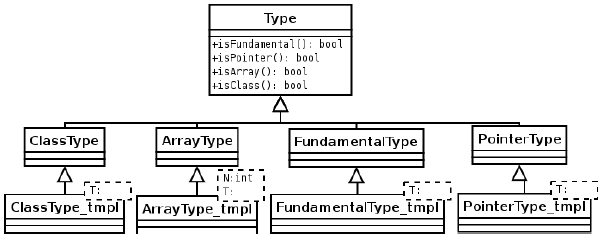
\includegraphics[width=0.5\linewidth]{ClassType.png}
    \caption{Metaclass hierarchy}
    \label{fig:ClassType}
\end{figure}

\begin{figure}
    \centering
    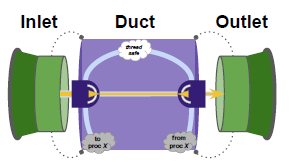
\includegraphics[width=0.5\linewidth]{Conduit.png}
    \caption{Conduit Scheme}
    \label{fig:Conduit}
\end{figure}
\clearpage
\printbibliography\end{document}
